\section{Transparency Plane}
If a user is moving his finger, while it is strapped in the device, he/she should perceive the device as little as possible. This is called \emph{transparency}. In this test we are interested to measure the torque, that has to be exerted by the user, in order to move the end-effector at a certain velocity or acceleration. This allows for a calculation of apparent inertia and damping according to the following equation:

\begin{equation}
    \tau_{user} = i*\dot \theta + b*\ddot \theta
\end{equation}

We want these values to be as small as possible.

\subsection{Implementation}

In this test, we want to measure the torque exerted by the user, therefore the system has to remain unactuated during the process. It is a very simple program that just records all measured data by the system. The velocity is measured once from the tacho and once as the derivation of the encoder signal.

To simulate a real usage of the device, the test-person should attach the index-finger and also use the normal handle. After starting the recording of the signals, the user has to move the finger in sine-form with different frequencies, in order to cover a broad spectrum. Alternatively, one can also move the end-effector by hand, which results in nicer, more even plots. 

\subsection{Data Analysis}

For data analysis we use the encoder derivative for the velocity and adjust the force signal with a leverarm of 7cm to determine the user torque. The same strategy was also used by Marc in his master's thesis \cite{marc}. Afterwards, the recorded signals are filtered with a butterworth low-pass filter with cutoff frequency 20Hz. Based on the filtered velocity signal, the acceleration is calculated by dividing the time-steps and velocity steps between two consecutive measurements.

After the data preprocessing, the measured user torques can be plotted over velocity and acceleration in a 3D plot as introduced in \cite{metzger}. These points are then approximated with a 3D-Plane. The plane is calculated with a minimize function, which minimizes the z-error between the plane and the measured torques. The plane has the following form:

\begin{equation}
    \tau_{user} = i_{app}*\ddot \theta + b_{app}*\dot \theta
\end{equation}

Therefore, the apparent inertia ($i_{app}$) and the apparent damping ($b_{app}$) can be directly read from the plane. Additionally, the average z-residual (error between measured points and plane) and the maximum z-residual are calculated to make a statement about the accuracy of the estimated inertia and damping.

\subsection{Results}

In the following, the transparency planes for MIKE \#6 and MIKE \#3 are shown. The velocity and acceleration range was chosen as Marc did in his report, in order to have a comparable operating range for all MIKE versions. In addition to the plots, the apparent inertia ($i_{app}$), the apparent damping ($b_{app}$) as well as the average ($r_{avg}$) and the maximum ($r_{max}$) z-residual are indicated next to the plot. Both plots were recorded by moving the end-effector by hand and not with the finger attached. They show similar results to what was presented in Marc's report ($i_{app} = 0.0164\frac{gm^2}{deg}$ and $b_{app} = 0.242\frac{mNm}{deg/s}$). 

\begin{figure}[h]
    \begin{minipage}[m]{0.8\textwidth}
     \centering
        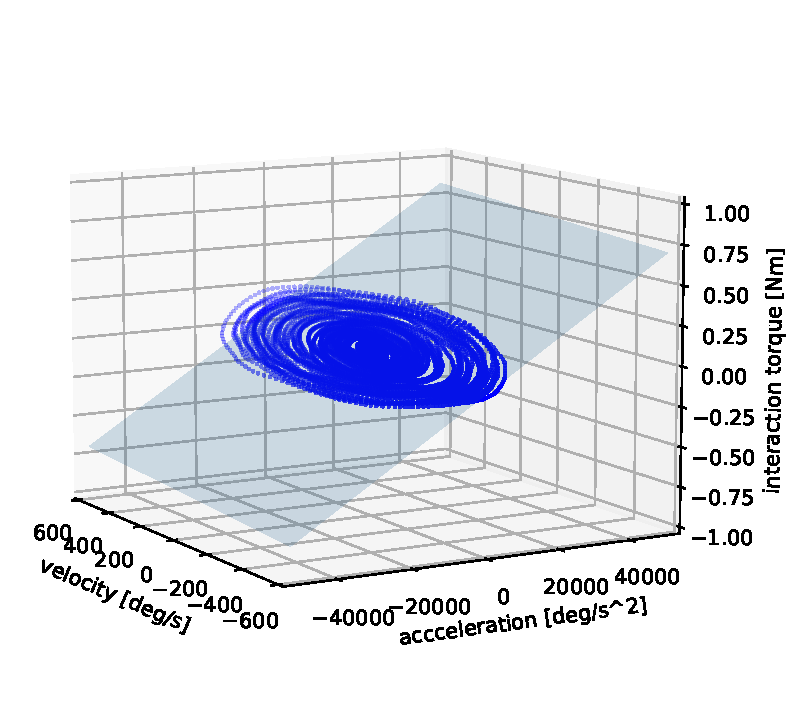
\includegraphics[width = \textwidth]{chapters/transparency/Mike6_Transparency.pdf}
    \end{minipage}
    \hfill
\begin{minipage}[m]{0.15\textwidth}
    \centering
    \begin{tabular}{lll}
        $i_{app}$ & = & 0.0149 $\frac{gm^2}{deg}$ \\ 
        $b_{app}$  & = & 0.1032 $\frac{mNm}{deg/s}$  \\ 
        $r_{avg}$  & = & 0.011 Nm \\
        $r_{max}$  & = & 0.0489 Nm \\ 
    \end{tabular}
\end{minipage}
\caption{Transparency Plane of ETH MIKE \#6}
\end{figure}

\begin{figure}[h]
    \begin{minipage}[m]{0.8\textwidth}
     \centering
        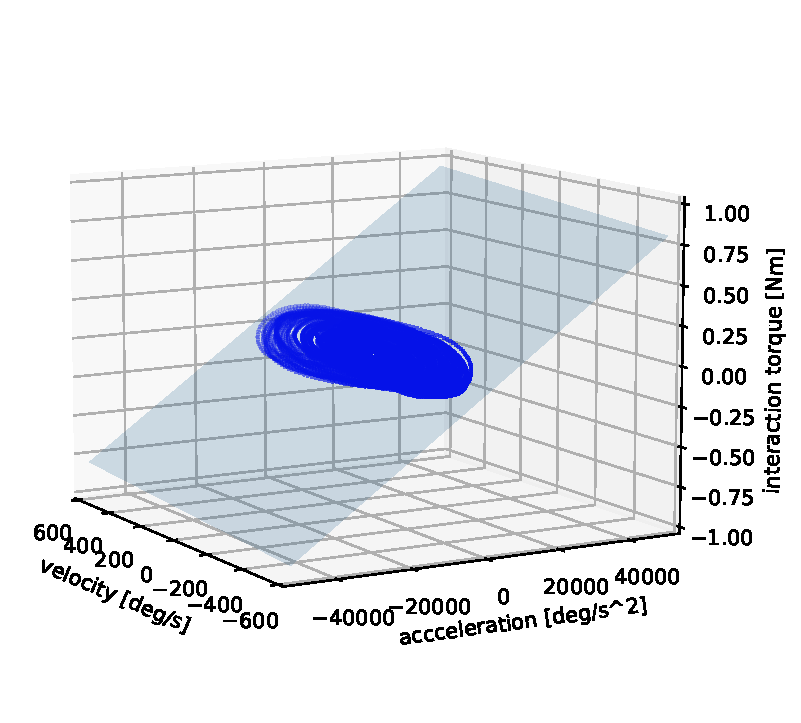
\includegraphics[width = \textwidth]{chapters/transparency/Mike3_Transparency.pdf}
    \end{minipage}
    \hfill
\begin{minipage}[m]{0.15\textwidth}
    \centering
    \begin{tabular}{lll}
        $i_{app}$ & = & 0.0171 $\frac{gm^2}{deg}$ \\ 
        $b_{app}$  & = & 0.113 $\frac{mNm}{deg/s}$  \\ 
        $r_{avg}$  & = & 0.0125 Nm \\ 
        $r_{max}$  & = & 0.0716 Nm \\ 
    \end{tabular}
\end{minipage}
\caption{Transparency Plane of ETH MIKE \#3}
\end{figure}